\documentclass[twocolumn]{article}
\usepackage[english]{babel}
\usepackage{float}
\usepackage{url}
\usepackage[latin1]{inputenc}
\usepackage{datetime}
\usepackage{graphicx}
\makeatletter
\setlength{\@fptop}{0pt}

%%%%%%%%%%%%%%%%%%%%%% Title Page %%%%%%%%%%%%%%%%%%%%%%%%%%%%%%%
\begin{document}
\onecolumn
\begin{figure}[b!]
\centering

\includegraphics[keepaspectratio, width=0.3\textwidth]{./logo.png}
\end{figure}
\title{A Note on Cryptocurrency Stabilisation: Seigniorage Shares}
\usdate
\author{Robert Sams\\\texttt{robert@kryptonomic.com}}
\maketitle
\begin{abstract}
  Cryptocurrencies like Bitcoin govern the supply of coin through
  simple and \emph{deterministic} coin growth rules. As a result,
  unanticipated changes in coin demand are reflected in changes in
  coin price, causing volatility and discouraging usage of coin as
  media-of-exchange. We argue that next-generation cryptocurrencies
  should incorporate an \emph{elastic} supply rule that adjust the
  quantity of coin supply proportionately to changes in coin market
  value. There are two difficult problems to solve in order to
  implement such a scheme. This note outlines a solution to one of
  those problems, and offers some suggestions on how the other problem
  might be solved.
\end{abstract}
\titlepage


%%%%%%%%%%%%%%%%%%%%%% Content %%%%%%%%%%%%%%%%%%%%%%%%%%%%%%%
\twocolumn
%\tableofcontents
\section*{Coin Supply and Volatility}
Cryptocurrencies like Bitcoin govern the supply of coin through simple
and deterministic coin supply rules. By ``deterministic'' I mean that
the growth rate of coin supply is completely specified in advance and
is not influenced by facts outside of the system.\footnote{This is not
  completely correct. Accelerating growth in the hashrate means that
  the average interval of block times is lower than the 10 minutes
  targeted by Bitcoin's difficulty adjustment rule. But this
  influence is marginal.} This is a significant departure from even
pure commodity money systems, as the supply of a precious metal is
responsive to price changes that cross the marginal cost of pulling
the stuff out of the ground.

If a cryptocurrency system aims to be a general medium-of-exchange,
deterministic coin supply is a bug rather than a feature. This is
because changes in coin demand get translated into changes in coin
price, making price volatility proportional to demand volatility. But
that is only a first order effect, for \emph{expectations} of future
levels of coin demand give rise to speculation. If the expectations of
the long-term rate of coin adoption are significantly greater than the
rate of coin supply growth, people will buy and hold coin in
anticipation of future adoption, driving up the current price of coin.

It is the nature of markets to push expectations about the future into
current prices. Deterministic money supply combined with uncertain
future money demand conspire to make the market price of a coin a sort
of prediction market on its own future adoption. Since rates of future
adoption are highly uncertain, high volatility is inevitable, as
expectations wax and wane with coin-related news, and the coin market
rationalises high expected returns with high volatility (no free
lunch).

The problem is that high levels of volatility deter people from using
coin as a medium of exchange. Given that the bullish case for
buy-and-hold coin speculation is based on expectations of substantial
medium-of-exchange usage in future, it might be conjectured that
deterministic money supply rules are self-defeating.

\section*{Coin Demand}
In light of this, it makes sense to analyse coin demand into two
types:
\begin{itemize}
\item Transactional Coin Demand $CD_{T}$
\item Speculative Coin Demand $CD_{S}$
\end{itemize}
Transactional coin demand is the desire to hold a certain quantity of
coins for the purpose of making transactions. You can think of
$CD_{T}$ as the sum of all coin balances held with such a
motive. Speculative money demand is the desire to hold a certain
quantity of coins in the expectation that its price will
appreciate. You can think of $CD_{S}$ as the sum of all coin balances
held as part of a portfolio of savings. 

A given individual is likely to possesses both speculative and
transactional motives for holding coin and he may not even mentally
demarcate his coin balance to reflect the different motivations. But
for analytical and empirical purposes, it makes sense to model coin
demand as if he does and analyse aggregate coin demand as:
\begin{equation}
CD = CD_{T} + CD_{S}
\end{equation}
In macroeconomic research, speculative demand for a fiat currency is
often conjectured to be driven by factors such as the level of
interest rates and the degree of risk aversion over risky assets. But
coins are different. Because they are young and the potential growth
rate of adoption is substantial, coins are among the most volatile of
assets. What drives speculative demand is anyone's guess. On the most
charitable, rational-expectations analysis, $CD_{S}$ is driven by
expectations of future levels of $CD_{T}$. Less charitably, it is
driven by the evolution of the coin price itself, trend-following
behaviour and ``greater-fool'' beliefs.

The problem is that $CD_{T}$ itself is negatively influenced by the
level of volatility in coin price. Enthusiasts and early-adopters
notwithstanding, most people prefer to hold stable medium-of-exchange
over volatile media simply because they are risk-adverse with respect
to wealth. I think the socio-economic make-up of the cryptocurrency
community (primarily educated and affluent) under-estimates the
relevance of risk-aversion to money demand. The poorer you are, the
higher percentage of your wealth is held in money, and when
entertaining prospects of mass adoption, it's important to reflect on
the reasons for why the Gini coefficient over money is lower than Gini
coefficient over total wealth.

And risk aversion isn't the only reason for why we should expect
$CD_{T}$ to be inversely related to the volatility of coin
price. Volatility also generates transaction costs. Substantial
declines in coin price require the conversion of fiat currency into
coins, and substantial increases in coin price require conversion of
coins into fiat currency (or some other asset) in order to maintain
the desired balance of coin purchasing power. Both the
\emph{frequency} of such re-balancing, and the
\emph{cost-per-transaction} of each re-balancing are correlated with
coin volatility.

\begin{figure}
  \begin{center}
    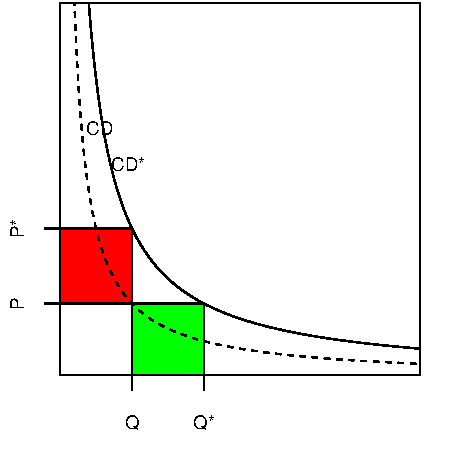
\includegraphics{chart1.pdf}
  \end{center}
  \caption{Money Demand}
  \label{fig:money-demand}
\end{figure}

Coin demand is a quantity of \emph{purchasing power} rather than a
quantity of coin. That is,
\begin{equation}
CD = P\times Q
\end{equation}
, where P is a coin's purchasing power (coin price of a basket of
goods and services) and Q is the quantity of coins demanded with
respect to a given coin price. Unlike the demand curve for ordinary
goods, where price elasticity is an empirical matter, the relationship
between quantity of coins demanded and coin price can be postulated
apriori as in $CD$ in figure \ref{fig:money-demand}. 

In a protocol like Bitcoin's, when money demand shifts e.g., from $CD$
to $CD*$, this results in a change in price from $P$ to $P*$, as
represented by the red box.

\section*{Elastic Coin Supply}
But in a coin stabilisation scheme, changes in coin price stand proxy
for changes in coin demand, and coin supply changes in response to
changes in coin price. The idea is that an $X\%$ change in coin price,
followed by an $X\%$ change in coin supply, will return coin price to
its initial value, as as represented by the green box.

So the core operational principle of a protocol that aims to stabilise
the market value of coin is the following rule: \textbf{at the end of
  some pre-defined interval of time, if the change in coin price over
  the interval is $X\%$, change coin supply by $X\%$.}

More specifically, let's call that interval of time the \emph{rebase
  period}, defined as every $n$ blocks. The coin supply rule mandates
that:
\begin{eqnarray}
Q_{i} &=& Q_{i-1}\times \frac{P_{i}}{P_{i-1}}\label{eqn:supply}\\
\Delta_{i} &=& Q_{i} - Q_{i-1}\label{eqn:delta}
\end{eqnarray},
where $i$ is the i-th rebase period, $Q$ is coin supply and $P$ is
coin price. 

\subsection*{Two hard problems}
How do we actually implement such a scheme in a cryptocurrency? There
are two hard problems to solve here:
\begin{enumerate}
\item How can $P_{i}$ be represented inside the network in a way that
  requires minimal trust?
\item How is $\Delta_{i}$ distributed? 
\end{enumerate}
The first problem is hard because however the protocol defines $P_{i}$
(it may be defined as the coin price of an index of commodities,
consumer goods.. or simply the USD price of coin), the variable will
be a fact about the world outside the system that needs to be
represented inside the system via some trust-minimising
mechanism. What kind of mechanism can have that property is
non-obvious, to say the least. We will discuss some strategies for
solving this problem in section at the end of this note, but that
problem isn't the focus of this note.

Here we are going to outline a solution to the second problem. Most
cryptocurrency systems only increase coin supply, and distribution is
done via the mining award. But in a stabilisation scheme, even if
$E[\Delta_{i}]$ is positive, there are times when $\Delta_{i}$ is
negative, and coin stabilisation needs a mechanism for \emph{reducing}
the coin supply as well as increasing it, so the mining award channel
isn't a solution to the problem of how $\Delta_{i}$ is distributed.

\section*{How \emph{not} to distribute $\Delta_{i}$}
One simple solution is to distribute $\Delta_{i}$ pro-rata over all
coin balances. This is the approach advocated by Ametrano in his
creative coin stabilisation scheme dubbed "Hayek
Money''\cite{ametrano}. This approach has the virtue of
simplicity. All wallet balances are simply multiplied by $Q_{i} /
Q_{i-1}$ in each period to arrive at a new wallet balance. This is
very easy to implement technically, the protocol just stipulates the
calculation of a rebase factor that is included in each block
header. (I think that this is how Friecoin implements its demmurage
rule.) It may seem a little awkward that the nominal value of one's
wallet fluctuates with changes in money demand, but that might be a
tolerable price to pay for a system that achieved coin price stability.

The problem is that this scheme only stabilises \emph{coin price}, it
doesn't stabilise the \emph{purchasing power} of a wallet
balance. Recall the three functions of money:
\begin{enumerate}
\item Unit-of-Account
\item Store-of-Value
\item Medium-of-Exchange
\end{enumerate}
Price stability is not only about stabilising the unit-of-account, but
also stabilising money's store-of-value. Hayek money is designed to
address the former, not the latter. It merely trades a fixed wallet
balance with fluctuating coin price for a fixed coin price with
fluctuating wallet balance. The net effect is that the purchasing
power of a Hayek Money wallet is just as volatile as a Bitcoin wallet
balance. So the self-defeating dynamic of $CD_{S}$ driving out
$CD_{T}$ remains.

\section*{Seigniorage Shares}
The solution to coin distribution offered here is different. I suggest
that there needs to be two types of coin: coin that acts like money
and coin that acts like shares in the system's seigniorage. For short,
we'll just call these \emph{coins} and \emph{shares}. Coins and shares
are identical in all respects (transaction verification works via
ECDSA signature, etc) except for the process that regulates their
respective supply.

Coins are the object of stabilisation, and $\Delta_{i}$ of coin is
distributed to the holders of shares. When coin supply needs to
increase, coinbase is distributed to share holders in exchange for a
certain percentage of shares, which are destroyed (coin supply
increases, share supply decreases). When coin supply needs to
decrease, sharebase is distributed to coin holders in exchange for a
certain percentage of coin, which are destroyed (coin supply
decreases, share supply increases). 

The mechanism of these shares-for-coin and coin-for-shares swaps is a
voluntary one, a decentralised auction the rules of which are written
into the protocol. The quantity of coins to create or destroy is
defined via the $\Delta_{i}$ process in equations \ref{eqn:supply} and
\ref{eqn:delta}, and there is an auction at the end of every rebase
period. 

When $\Delta_{i}$ is positive (new coins need to be created) a
\emph{coin auction} for $\Delta_{i}$ coins begins at the block or
ledger set defining the start of rebase period $i+1$. Any holder of
shares can bid for coins by signing and broadcasting a special TX
describing the quantity of shares he is willing to trade for coin, and
the \emph{minimum} coins/shares price that he will accept. Winning
bids are filled at whatever coins/shares price $P^{s}$ that clears the
quantity to be sold. So $\Delta_{i}$ new coins are distributed to the
winning bidders and $\Delta_{i}/P^{s}$ shares are destroyed via
proof-of-burn.\footnote{Defining the exact details of a decentralised
  auction is of course a subject in itself. In order to prevent
  front-running by validating nodes, the auction will have to take
  place over three periods. In the first period, bids are hashed and
  broadcast, and consensus is achieved on the existence of the
  encrypted orders. In the second period, bidders will broadcast the
  unencrypted order contents and nonce, and consensus is achieved on
  those by validating that the submissions in the second period hash
  to the digests submitted in the first period. In the third period,
  validating nodes validate the spends and and apply the auction
  protocol to determine winning bids and $P^{S}$.}

When $\Delta_{i}$ is negative (some existing coins need to be
destroyed), a \emph{share auction} of $\Delta_{i}$ \emph{worth of
  shares} begins. Holders of coin can submit bids to purchase shares,
signing a special TX describing the quantity of coins he is will to
trade for shares, and the \emph{maximum} coins/shares price $P^{s}$
that he will accept. Winning bids are filled at whatever price clears
the quantity to be sold. So $\Delta_{i}/P^{s}$ new shares are
distributed to the winning bidders and $\Delta_{i}$ coins are
destroyed via proof-of-burn.

If the long-run demand for coin is positive, coin supply will increase
with demand, but the quantity of shares will get increasingly
scarce.

\section*{Valuing Seigniorage Shares}
At first this scheme looks exotic, as if we need some model of
``scarcity value'' in order to estimate a fair value shares. But this
isn't the case at all, for a position in shares is really just a claim
on future coin supply growth and can be valued as if it were an
income-generating asset.

Consider the following investment strategy. When $\Delta_{i}$ is
positive, the investor sells $\Delta_{i}/(P^{s}_{i}Q^{s}_{i})$ percent
of his position in the auction; when $\Delta_{i}$ is negative, he
increases his position by that percentage by buying shares in the
auction. As a result, the investor maintains a position in a
\emph{fixed percentage} of the outstanding share supply and therefore
has a claim on that fixed percentage of $\Delta_{1}, \Delta_{2},\dots$
in perpetuity. Therefore, the price of shares is nothing more than the
Net Present Value of that income stream. So share price at time $t$
is:

\begin{equation}
\label{eqn:npv}
P^{s}_{t} = \frac{1}{Q^{s}_{t}}\sum\limits_{i=t}^{\infty}\frac{\Delta_{i}}{(1+r_{i})^{i}}
\end{equation}

, where $r_{i}$ is the discount rate applied to the seigniorage $i-th$
periods in future. 

As with any NPV analysis, $r_{i}$ must be above the growth rate of
$\Delta_{i}$ for the series to converge to a finite value, and both of
those variables are of course subjective forecasts of market
participants. As with any market in cash flow perpetuities (eg,
stocks), valuation metrics can be devised that calibrate forecasts of
these variables to historical series of $\Delta_{t}$ and $P_{t}$. 

If the coin is designed along the lines of a proof-of-work blockchain
with a block award, then the numerator in the summation term will
need to instead be $\Delta_{i} - \alpha_{i}(N)$, where $\alpha$ is the
block award in coin and $N$ is the number of blocks in the rebase
period. Stable coin schemes have the nice side-effect that the market
value of the block award (and therefore, its contribution to to
network security) can be defined explicitly, instead of fluctuating
with the price of coin, as is the case with a protocol like Bitcoin.

With this dual model of coins and shares, speculators now have a
market that they can actually \emph{value}, and we can now exploit the
dual motivations for money demand; coins are the object of $CD_{T}$,
shares are the object of $CD_{S}$, and the Janus-faced nature of $CD$
can work in harmony like a monetary ying and yang rather than $CD_{S}$
chasing away $CD_{T}$, as is the case with monocoin schemes with
deterministic coin supply rules.

\section*{Decentralised Monetary Policy}
Critics of central banking (and I am among them) too often extend
their criticism of the institutional failures of centralised and
discretionary monetary policy to the very concept of monetary policy
itself. 

Any monetary regime has a monetary policy. A commodity money regime
like a gold-standard has a monetary policy dictated by the cost of
pulling new supply of the commodity out of the ground. It has the
virtue of a being a monetary policy driven by rules rather than human
discretion. But it has the downside of fixing the supply function to
an arbitrary process--cost of mining gold--that may not serve the goal
of stabilising the purchasing power of money particularly
well. Bitcoin has a monetary policy too, but it's arguably worse than
the monetary policy of commodity money, as its supply function isn't
influenced by the value of Bitcoin at all.\footnote{except at the
  margin, when non-linear growth in network hash power causes block
  intervals to average below 10mins.}

In a sense, this dual model of coins and shares embodies the
functionality of a fiat money central bank--without the
centralisation, or the bank\footnote{Even calling central banks
  "banks" is an anachronism, homage paid to their historical
  evolution, for in the current fiat money world, a central bank is
  unique in being the only institution where the "liability" side of
  its balance sheet is a liability in name only; fiat money isn't a
  claim on anything, by definition, and the holders of national bank
  notes are not creditors of the central bank like the holders of a
  bank deposit are a creditors of a commercial bank.}. Setting aside
the complexity of monetary policy transmission in an economy with
fractional reserve banking, the essence of a central bank's operations
is the use of its balance sheet to adjust the supply of money. Money
supply is expanded by purchasing assets with newly created
money. Money supply is decreased by selling assets, thereby
extinguishing part of the money supply. For all the mystique that
surrounds central banking, and the current fashion for targeting
interest rates rather than money supply, this is the essence of what a
central bank does.

In this way, a central bank can increase the money supply without
limit. But its ability to shrink the money supply is constrained by
the value of the \emph{assets} it holds. Seigniorage shares are like
the asset side of a central bank's balance sheet. The market
capitalisation of shares at any point in time fixes the upper limit on
how much the coin supply can be reduced.

\section*{Solving the Other Problem}
So far we have just assumed that our network has a mechanisms for
achieving consensus consensus on what $P_{i}$ is. This is a separate
hard problem in its own right. Here's a brief sketch on how I think
this problem might be solved. 

Firstly, I think that there are two families of design here, one that
works with \emph{exogenous} data sources for $P_{i}$ and a more
restrictive strategy that defines $P_{i}$ in terms of information that
is purely \emph{endogenous} to the network itself.

Without specifying what types of values $P_{i}$ could be, we've sort
of assumed the \emph{exogenous} design in this note. That is, $P_{i}$
would be defined as some specific price index. What that index is
would be specified at the time of the scheme's launch, and the
motivation would be some price index that we want to make coins stable
\emph{with respect to}. For example, maybe the USD price of coin,
deflated by the CPI, for ``zero-inflation'' coin. 

\subsection*{Schelling Points}
The best strategy I am aware of for solving this problem for exogenous
designs is a schelling point scheme. The goal is to have a mechanism
to incentivise people to submit accurate estimates of $P_{i}$ to the
network. 

One mechanism for doing this is to have a periodic competition, where
people submit encrypted estimates of $P_{i}$ to the network, along
with $F$ coins, the price for participating in this mechanism. The
incentive for participating is that after all the submissions are
collected and decrypted, everyone who submitted a value inside the
inner two quartiles of the estimate distribution wins $2\times F$,
whilst all those with estimates in the outside two quartiles lose
$F$. So the incentive is to bet what you think the consensus will be. 

The idea here is that the ``rational'' expectation of what consensus
will be is whatever is common knowledge of the \emph{salient}
answer. A Schelling point is a qualitative equilibrium solution based
on common knowledge of salience and in our context, the hope is that
\emph{truth} is the Schelling point.

Various suggestions along these lines have been suggested before by
Sams\cite{sams}, Buterin\cite{buterin}, Ametrano\cite{ametrano} and
probably others. I'm still uneasy about the robustness of the
truth-as-schelling-point assumption, especially given the potentially
complex interaction of incentives outside and inside the schelling
point mechanism.

But perhaps more structure can be placed on the Schelling scheme by
restricting participation to share holders. If my primary empirical
conjecture that $CD_{T}$ is inversely related to coin price
volatility, maybe it can be shown that the price of shares as defined
by equation \ref{eqn:npv} is maximised by whatever set of estimated
coin prices $P_{i}$ most accurately represents the basket of
goods/assets that coin holders want coin to be stable against. In
other words, maybe by restricting participation in the Schelling
mechanism to share holders, the union of incentives of share holder
and Schelling game participant are more likely to bring about a
process where the Schelling point is truth. And $P_{i}$ will then be
the coin price of a representative basket of goods that coin holders
typically use coin to buy, a sort of coin CPI, and it's up to share
holders to come to consensus (via iterations of the Schelling game) of
what that coin CPI actually is. 

\subsection*{Endogenous models}
An entirely different strategy is that which I call an endogenous
stabilisation model. Stabilising coin with respect to the coin market
value of some index of goods/assets isn't the only form that
stabilisation can take. The goal isn't indexing per-se, but stability
itself. As we intimated in the previous section, what coin should
ideally be stable against isn't necessarily a known parameter and can
change through time. But throughout this note we have implicitly
defined ``stability'' in a relative sense, stability with respect to a
price index. But why not make the goal some notion of robust
stability, a coin that is usually stable with respect to any randomly
selected, broad index of goods/assets.

And perhaps information endogenous to the protocol itself is
sufficient to achieve this more general goal. If the coin is based on
a proof-of-work blockchain, two candidate variables stand out: the
average level of \emph{transaction fees} and hashing
\emph{difficulty}. Now what information these two variables contain
about the outside world depends upon what particular fee model and
hashing algorithm the protocol defines. But I believe they do contain
information relevant to coin stability. 

Fees. If there is no block size limit, or the limit doesn't generally
force miners to ration transaction inclusion, then we can postulate
that fees will converge to the average cost of validating transactions
times N, the number of validating nodes. So holding constant the
computational cost of transaction validation, it stands to reason that
changes in average fee levels signal either changes in coin value
and/or changes in N.

Difficulty. Similar pattern. Holding GHs/kWh constant, a change in
difficulty signals change in coin value, as hashing power is turned
on/off until hashing costs equal the market value of mining award. 

The market information contained in these two variables has been
hugely obscured by the explosive progress in hardware optimisation of
hashing. But is it not reasonable to think that rates of optimisation
will slow down to roughly predictable levels and eventually be
governed by the same constraints (photo-lithography, etc) that CPU and
GPU design is subject to? 

If so, perhaps the most robust solution is to define $P_{i}$ in terms
of fees and difficulty, deflated by some hard-coded Moore's Law-like
assumption. This would avoid the need to represent market facts about
the outside world at all, keeping the stable coin scheme autonomous
and self-referential. 

But all of these suggestions for tackling problem 1 are speculative
and I have no convictions here whatsoever. This is a hard problem.

\begin{thebibliography}{9}
\bibitem{ametrano}
Ferdinando M. Ametrano,
  \emph{Hayek Money: The Cryptocurrency Price Stability Solution
    (August 19, 2014)}.
Located at \url{http://ssrn.com/abstract=2425270} or
\url{http://dx.doi.org/10.2139/ssrn.2425270}
\bibitem{buterin}
Vitalik Buterin, \emph{SchellingCoin: A Minimal-Trust Universal Data Feed (March 28,
  2014)}. Located at
\url{https://blog.ethereum.org/2014/03/28/schellingcoin-a-minimal-trust-universal-data-feed}
\bibitem{sams}
Robert Sams, \emph{What would a trusted data feed look like (February 5,
  2014)[Reply to forum posting]}. Located at \url{https://forum.ethereum.org/discussion/31/what-would-a-trusted-data-feed-look-like/p1}
  \end{thebibliography}
\end{document}
 
